\chapter{Problem definition}
One edge of Medialogy is systems built to react accordingly to humans. This system is called Visual Computing. There are several not least good topics that apply to this kind of technology. One area in which image processing and specific object recognition is used, is surveillance. By implementing some custom made software, one will be able to monitor a specific target group or process. In addition to the semester project two mandatory courses on the third semester of Medialogy are of interest to our semester project.\\
The first course is called Image Processing and it's primarily based on understanding, the theory of a picture and tools to manipulate the pixel values within. knowledge such as the princip of 8-bit, the RGB color system, histograms and using thresholding to segmentate a picture are some tools learned in the course.\\
The second course used for the semester project is Procedural Programming, in which programming skills in C++ are learned. The theoretical bagground for programming is necessary to complete image manipulations, based on methods learned in Image Processing.

To structure the semester projects considering supervisiors and co-supervisors, every group was asked to discuss which subject field that was of interest to them. In continuation of this every group was asked to submit an application fo the three subjects of the biggest interest, with first, second and third priority.\\
The eleven subjects presented was:

\begin{itemize}
\item Image Processing for Fun Utilizing an Industrial Robot
\item Image Processing for Ambient Intelligent Robots
\item Interactive Floor
\item Interactive Book
\item Interactive Drawing Game
\item Interactive Arcade Game
\item Mobil app for recognizing electric components
\item Emergency system for old people that have fallen
\item Thermal Sock Puppet Show
\item Body Motion Controlled Exercise Game
\item Hjørring Library
\end{itemize}

In continuation of the last subject "Hjørring Library", three groups each year on the third semester of Medialogy is selected to collaborate with Hjørring Library in creating some intuitive interface that will react to humans. It was decided within the group that it was of interest to work with Hjørring Library, therefore an application was sent to the semester coordinator to consider our group as one participant. This was the first priority of our group.

As only three groups on the third semester applied for working with Hjøring Library, our group was chosen. A meeting was arranged with Hjørring Library and so together with 5 other groups from third and fifth semester of Medialogy, all groups traveled to Hjørring to meet some of the staff. In addition the groups were let loose in the library to check locations for potential projects.\\
After talking to some of the staff, more specific our contact person Martin Jørgensen. Some generals ideas emerged, so it was decided to go back to the group room at Novi to do some brainstorming within the group.

The first idea that emerged, included scanning of bar-codes of books in the library. The idea was that the shade of people trespassing the walkway wher the canvas was placed, would be projected onto the canvas. The conceptual idea was that people would explore the library and depending on the book gathered and loaded, some specific graphic would appear on the canvas, such as a fairy tale from H.C. Andersen that would produce a hat on-top of the user.

After conferencing with the supervisor Thomas Moeslund and the co-supervisor Andreas Møgelmose, it was decided that the conceptual idea needed to be narrowed down to a more specific subject field. The second idea emerged that we should focus mainly on fairy tales and first of all work around H.C. Andersen, which meant adding a hat on-top of the users.

An email was sent to "Martin Jørgensen" concerning the concept for the third semester project and also the location of the project. Martin liked the idea, but had some concerns to identify the period in which the project would fit the library. Hjørring Library work around specific topics that change every 8-12 weeks. One of the upcoming themes of interest at the library was Christmas that would run from the 2nd week in November until the last week of December. Another idea then emerged in the group towards creating a project for December. Instead of working with the H.C. Andersen theme, it was decided to work with father Christmas and to add a Christmas hat on-top of trespassing users of the library. Martin was fond of this idea and so a new meeting was arranged in order to settle on a suitable location at the library for our project.\\
Two members of the group traveled to Hjørring Library to participate in the meeting with Martin. The outcome was a more specific plan on the project concerning the:
\begin{itemize}
\item The position of the project
\item The equipment that was desired to borrow
\item The light conditions
\end{itemize}
The position of the project will be on the walkway from the reception desk to the core of the library, which Martin believed would be an ideal position for the project, as the light conditions are controllable. In addition to that he knew from experience that people tend to use that walkway either to enter or exit the library, as it is the shortest route.

\begin{figure}[htbp]
\centering
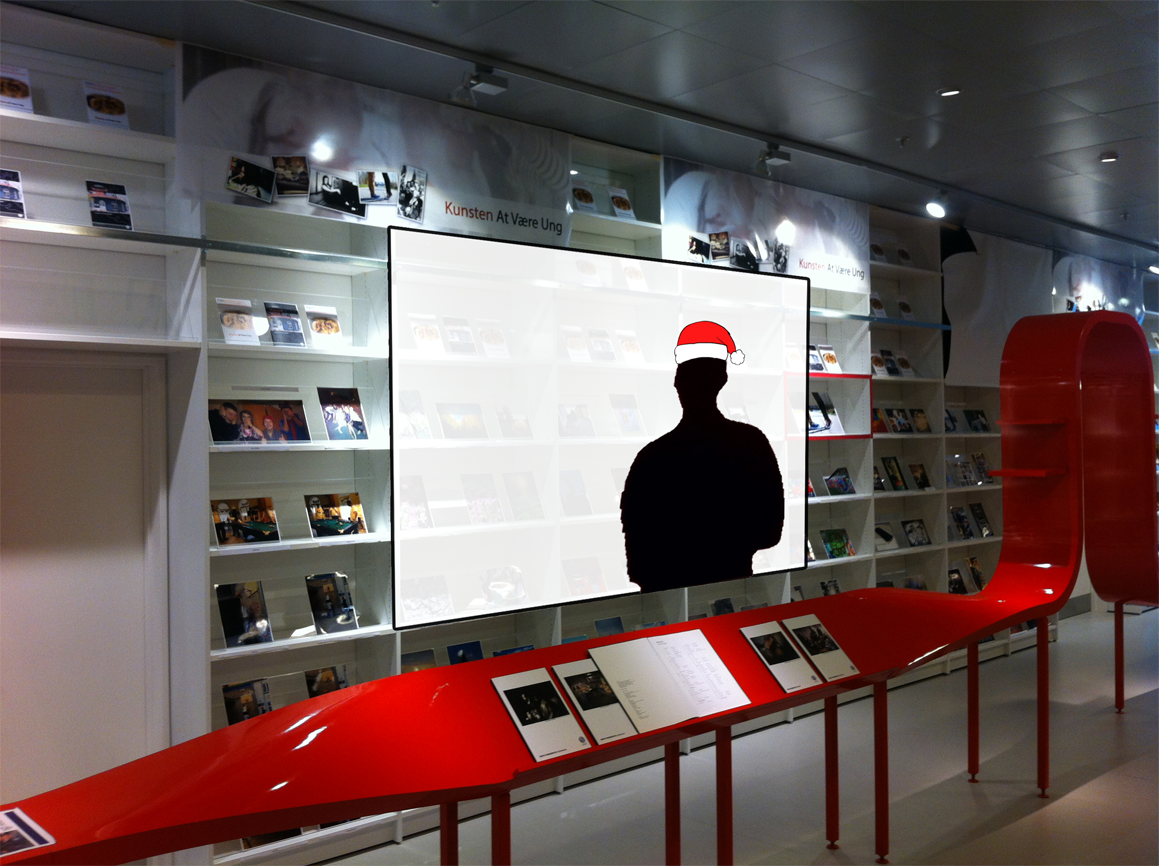
\includegraphics[width=1.00\textwidth]{Pictures/HjoerringLibrary/LocationJohannesHat.jpg}
\caption{Location at Hjørring Library}
\label{fig:Location at Hjørring Library}
\end{figure}

The picture above illustrates the setup at the library. A canvas with the proportions 3*2.25 meters will be positioned directly on the bookshelves seen in the background of the picture.

\textbf{Technical Point of view}\\
Together with a projector capable of projecting a relative huge output 3*2.25 meters, the laptop running the program code will also be connected to a webcam, modified to collect inferred lightning. This works by having some old lamps 


     


\section{This is awesome}
Yep yep

\begin{figure}[htbp]
\centering
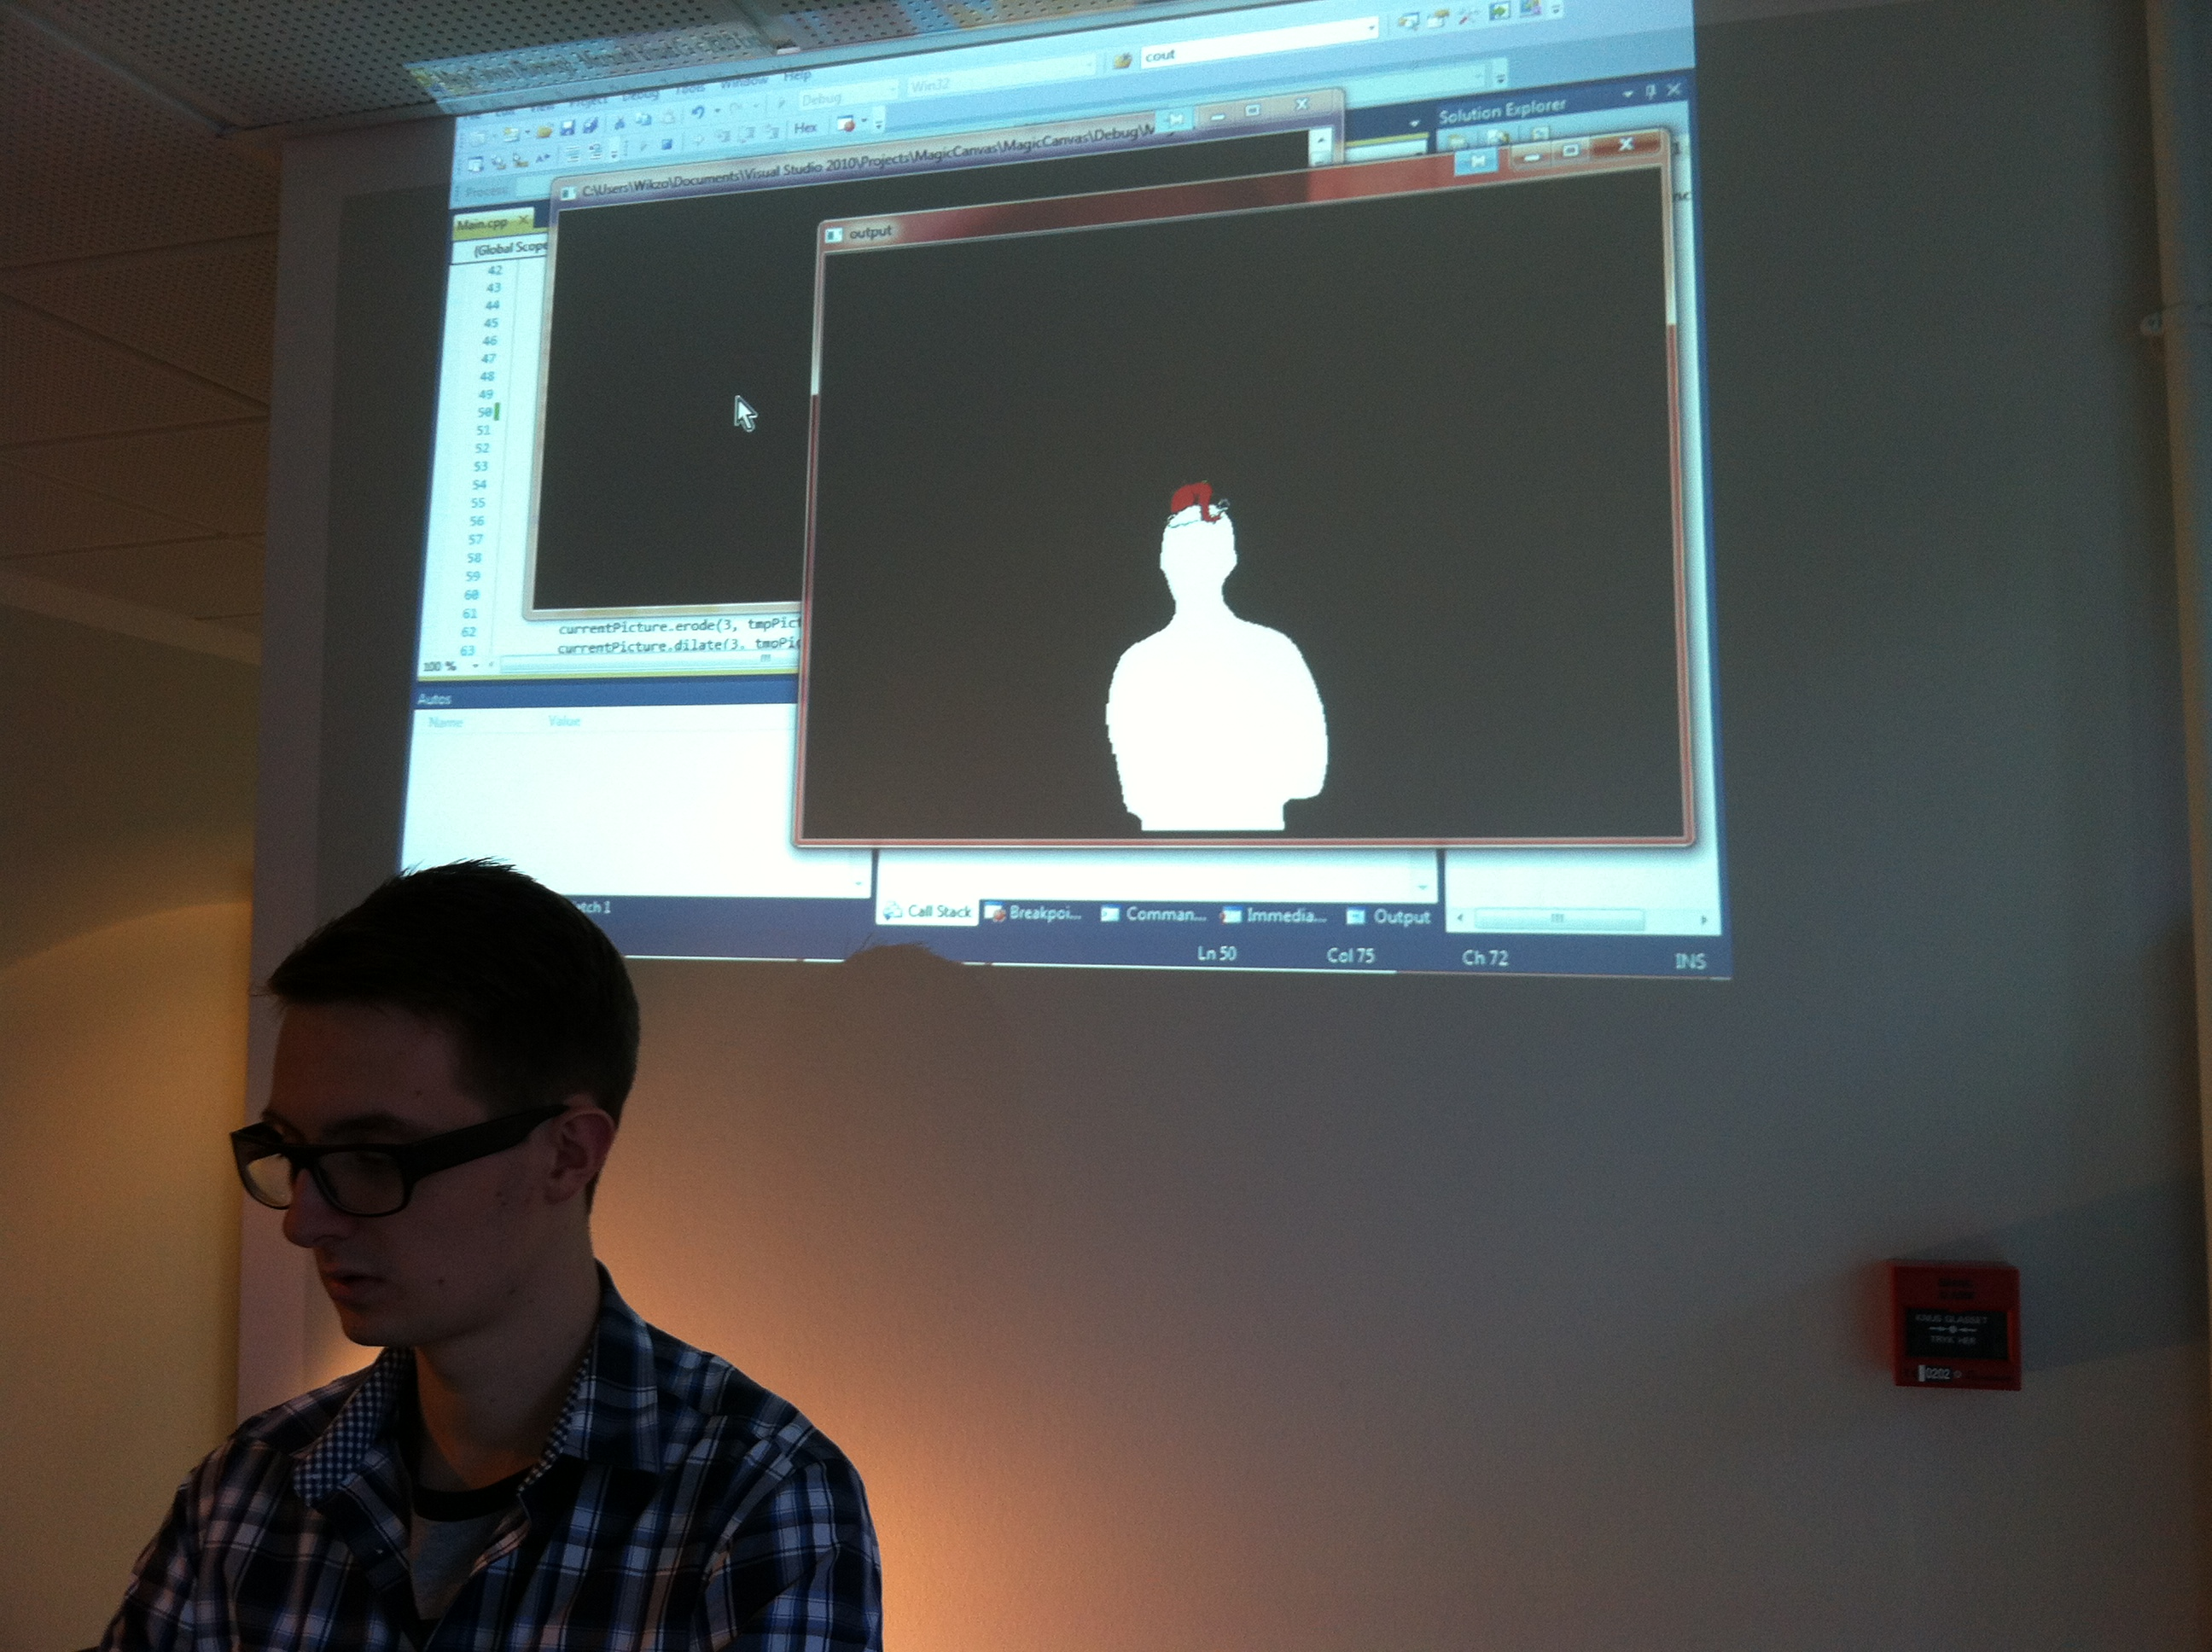
\includegraphics[width=1.00\textwidth]{Pictures/Test/IMG_1477.jpg}
\caption{Picture from Testing the Inferred Camera}
\label{fig:Picture from Testing the Inferred Camera}
\end{figure}

\subsection{Subway is good}
Nah...